\documentclass[12pt,letterpaper]{article}

% ── Packages ─────────────────────────────────────────────────
\usepackage[margin=1in]{geometry}
\usepackage{amsmath,amssymb,amsthm,mathtools}
\usepackage{thmtools}
\usepackage{array,booktabs}
\usepackage{xcolor}
\usepackage{hyperref}
\usepackage{fancyhdr}
\usepackage{titlesec}
\usepackage{enumitem}
\usepackage{tcolorbox}
\tcbuselibrary{breakable,skins,theorems}
\usepackage{mdframed}
\usepackage{tikz}
\usetikzlibrary{arrows.meta,positioning,matrix,decorations.pathreplacing}
\usepackage{float}
\usepackage{caption}
\usepackage{cleveref}

% ── Hyperref ─────────────────────────────────────────────────
\hypersetup{
  colorlinks=true, linkcolor=blue!65!black,
  citecolor=green!50!black, urlcolor=blue!60!black,
  pdftitle={QMHES Mathematical Appendix},
  pdfauthor={R. Van Gelder, Multiplicity Foundation}
}

% ── Headers ──────────────────────────────────────────────────
\pagestyle{fancy}
\fancyhf{}
\lhead{\small QMHES — Mathematical Appendix}
\rhead{\small Multiplicity Foundation, 2026}
\cfoot{\thepage}
\renewcommand{\headrulewidth}{0.4pt}

% ── Section formatting ───────────────────────────────────────
\titleformat{\section}
  {\large\bfseries\color{blue!70!black}}{\thesection}{1em}{}
\titleformat{\subsection}
  {\normalsize\bfseries\color{blue!45!black}}{\thesubsection}{1em}{}
\titleformat{\subsubsection}
  {\normalsize\bfseries\color{gray!60!black}}{\thesubsubsection}{1em}{}

% ── Theorem environments ─────────────────────────────────────
\theoremstyle{plain}
\newtheorem{theorem}{Theorem}[section]
\newtheorem{lemma}[theorem]{Lemma}
\newtheorem{corollary}[theorem]{Corollary}
\newtheorem{proposition}[theorem]{Proposition}

\theoremstyle{definition}
\newtheorem{definition}[theorem]{Definition}
\newtheorem{example}[theorem]{Example}
\newtheorem{remark}[theorem]{Remark}
\newtheorem{assumption}[theorem]{Assumption}

% ── Custom proof box ─────────────────────────────────────────
\tcolorboxenvironment{proof}{
  blanker, breakable,
  left=5mm,
  before skip=10pt, after skip=10pt,
  borderline west={1pt}{0pt}{blue!30!black}
}

% ── Notation shorthands ──────────────────────────────────────
\newcommand{\M}{\mathcal{M}}
\newcommand{\T}{\mathcal{T}}
\newcommand{\F}{\mathbf{F}}
\newcommand{\calB}{\mathcal{B}}
\newcommand{\calL}{\mathcal{L}}
\newcommand{\opnorm}[1]{\left\|#1\right\|_{\mathrm{op}}}
\newcommand{\frnorm}[1]{\left\|#1\right\|_{F}}
\newcommand{\vecnorm}[1]{\left\|#1\right\|_{2}}
\newcommand{\HMAC}{\mathrm{HMAC\text{-}SHA256}}
\newcommand{\HKDF}{\mathrm{HKDF\text{-}SHA256}}
\newcommand{\SHA}{\mathrm{SHA\text{-}256}}
\newcommand{\R}{\mathbb{R}}
\newcommand{\C}{\mathbb{C}}
\newcommand{\N}{\mathbb{N}}
\newcommand{\Z}{\mathbb{Z}}
\newcommand{\eps}{\varepsilon}
\newcommand{\lam}{\lambda}
\newcommand{\rekey}{\mathtt{REKEY}}
\begin{document}
% ══════════════════════════════════════════════════════════════════════════════

% ── Title Page ─────────────────────────────────────────────────────────────────
\begin{titlepage}
\centering
\vspace*{1.5cm}
{\Huge\bfseries\color{blue!80!black}
  Quantum-Multiplicity Hybrid\\[0.4em]
  Encryption System\\[0.3em]
  (QMHES)
}\\[1.2em]
{\Large\itshape
  Comprehensive Technical Report \&\\
  Prior Art Defensive Publication
}\\[2em]
\hrule height 1.5pt
\vspace{1.5em}
{\large
  \textbf{Authors:} R.\ Van Gelder\\[0.4em]
  \textbf{Organization:} Multiplicity Foundation / PhaseMirror\\[0.4em]
  \textbf{Repository:} \href{https://github.com/MultiplicityFoundation/PhaseMirror-HQ}%
    {\texttt{MultiplicityFoundation/PhaseMirror-HQ}}\\[0.4em]
  \textbf{License:} Prime Materia / CC BY-SA 4.0\\[0.4em]
  \textbf{Publication Date:} April 25, 2026\\[0.4em]
  \textbf{Document Version:} 1.0
}\\[2em]
\hrule height 0.8pt
\vspace{2em}

\begin{defensebox}
\textbf{Purpose of Defensive Publication.}
This document is filed as a prior art defensive publication. Its purpose is to
place the described concepts, methods, protocols, and implementations into the
public domain as prior art, thereby preventing any third party from obtaining
patent protection over these ideas or any substantial equivalent thereof.
This publication is intended to be indexed by patent offices, academic
databases, and technical archives. All disclosures herein constitute prior art
as of the publication date stated above, under the Multiplicity 2024 framework
originated by R.\ Van Gelder (Prime Materia License / CC BY-SA 4.0).
\end{defensebox}

\vfill
\small\textit{This document was compiled from original technical
specifications, mathematical frameworks, engineering roadmaps, and
implementation artifacts developed within the QMHES / PhaseMirror-HQ project.}
\end{titlepage}

% ── Table of Contents ──────────────────────────────────────────────────────────
\tableofcontents
\newpage

% ══════════════════════════════════════════════════════════════════════════════
\section{Executive Summary}
% ══════════════════════════════════════════════════════════════════════════════

This report describes the \textbf{Quantum-Multiplicity Hybrid Encryption System
(QMHES)}, a novel cryptographic architecture developed under the Multiplicity
Foundation's PhaseMirror-HQ project. QMHES constitutes a four-layer security
stack that unifies:

\begin{enumerate}[leftmargin=2em]
  \item \textbf{Quantum-State-Based Security (QSBS)} -- a mathematical framework
    mapping classical binary data and quantum amplitudes into a unified frequency
    space, secured via a dynamic, state-adaptive hashing operator augmented by
    Multiplicity Theory primitives (multiplicity operator $\mathcal{M}$, coupling
    tensor $\mathcal{T}$, non-linear feedback map $f$).

  \item \textbf{Quantum-Assisted Hybrid Encryption System (QAHES) v1.0.1} -- a
    byte-exact, wire-format transport protocol providing post-quantum key
    encapsulation (ML-KEM / CRYSTALS-Kyber, FIPS~203), post-quantum
    authentication (ML-DSA / CRYSTALS-Dilithium, FIPS~204), transcript-bound
    AEAD channels with per-direction replay protection, and a strictly specified
    handshake state machine.

  \item \textbf{Physical QKD Integration} -- a pluggable quantum key distribution
    adapter that sources information-theoretically secure key material via
    basis exchange, sifting, error correction, and Toeplitz-hash privacy
    amplification, confirmed via QBER monitoring and key pool management.

  \item \textbf{Multiplicity Theory Feedback Layer} -- a recursively stable,
    prime-indexed mathematical framework in which the multiplicity operator
    $\mathcal{M}_t$, coupling tensor $\mathcal{T}_t$, and non-linear feedback
    function $f$ govern adaptive key rotation, dynamic hash parameterization, and
    inter-subsystem entanglement integrity checks.
\end{enumerate}

\noindent
The system is partially implemented in Python within the
\texttt{packages/ace\_zk/} module family of
\href{https://github.com/MultiplicityFoundation/PhaseMirror-HQ}{PhaseMirror-HQ},
with \texttt{pq\_cert.py} providing the PQ signature abstraction (Dilithium5 /
SPHINCS+), \texttt{ffi.py} exposing a testable Python API, and
\texttt{daemon/audit.py} accepting post-quantum proof references in governance
ledgers. The engineering roadmap targets production readiness across multiple
deployment profiles (datacenter, metro fiber, satellite/FSO, embedded/HSM).

\bigskip
\begin{warnbox}
\textbf{Security classification of this novelty:}
The primary novel contribution of QMHES is the \emph{unified} architecture
combining (a) a frequency-space bridge between classical bits and quantum
amplitudes governed by Multiplicity Theory operators, (b) a byte-exact,
formally verifiable wire protocol with PQ and QKD key material, and (c) a
non-linear adaptive feedback mechanism that continuously adjusts cryptographic
parameters based on observable system state. No prior published system combines
all four layers in this manner.
\end{warnbox}

% ══════════════════════════════════════════════════════════════════════════════
\section{Background and Motivation}
% ══════════════════════════════════════════════════════════════════════════════

\subsection{The Post-Quantum Transition}

Classical public-key cryptography (RSA, ECDH, ECDSA) is vulnerable to
polynomial-time attacks by a sufficiently large quantum computer via Shor's
algorithm \cite{shor1994}. Grover's algorithm reduces symmetric key security by
a square-root factor. NIST finalized post-quantum standards in 2024:
ML-KEM (FIPS~203), ML-DSA (FIPS~204), and SLH-DSA (FIPS~205), based on
lattice hardness (Module Learning With Errors, MLWE) and hash-based
constructions.

\subsection{Limitations of Existing Hybrid Schemes}

Existing hybrid PQ+classical protocols (e.g., TLS~1.3 with kyber hybrid
groups) treat the PQ and classical layers as independent key agreements whose
outputs are combined via XOR or concatenation-then-KDF. They do not:
\begin{itemize}[leftmargin=2em]
  \item Incorporate \emph{adaptive} cryptographic behavior responsive to
    real-time system state, error rates, or threat signatures.
  \item Unify classical data representations and quantum mechanical state
    vectors in a common mathematical object that is secured as a whole.
  \item Use prime-indexed recursive structures to govern key rotation or
    entanglement integrity.
  \item Bind QKD key material into the same transcript-hash chain that governs
    PQ and classical AEAD operations.
\end{itemize}

\subsection{Multiplicity Theory}

Multiplicity Theory, originated by R.\ Van Gelder (Multiplicity 2024,
MIT/CC~BY-SA~4.0), is a prime-indexed, recursively stable mathematical
framework wherein \emph{multiplicity}---the recurrence of elements understood
through prime number decomposition---forms the basis for modeling nonlinear,
emergent structures. Mathematical objects are reinterpreted as recursively
generated patterns of prime-labeled interactions; sets and modules become
relationally governed multiplicity spaces with identity and behavior preserved
through recursive feedback loops across scales.

% ══════════════════════════════════════════════════════════════════════════════
\section{Comprehensive Mathematical Framework}
\label{sec:math}
% ══════════════════════════════════════════════════════════════════════════════

\subsection{Notation and Primitives}

\begin{definition}[Classical Payload]
Let $\mathbf{x} = (x_1, x_2, \ldots, x_n) \in \{0,1\}^n$ denote the classical
binary payload at time epoch $t$.
\end{definition}

\begin{definition}[Quantum State]
Let the quantum state be
\[
  |\psi\rangle = \sum_{j=1}^{m} \alpha_j |j\rangle, \qquad
  \alpha_j \in \mathbb{C}, \quad
  \sum_{j=1}^{m} |\alpha_j|^2 = 1.  \tag{1}
\]
The complex amplitudes $\alpha_j$ represent probability amplitudes over a
computational basis of dimension $m$.
\end{definition}

\begin{definition}[Multiplicity Operator]
The multiplicity operator $\mathcal{M}_t : \mathbb{R}^k \to \mathbb{R}^{k'}$
captures the dimensionality and complexity of the quantum state space at time
$t$. Concretely,
\[
  \mathcal{M}_t = \mathcal{M}\!\left(\|\psi_t\|,\; \varepsilon_t,\;
    \lambda_t,\; \mathrm{QBER}_t\right),  \tag{2}
\]
where $\varepsilon_t$ is the current bit-error rate, $\lambda_t$ is the
session load, and $\mathrm{QBER}_t$ is the quantum bit error rate of the QKD
channel.
\end{definition}

\begin{definition}[Coupling Tensor]
The coupling tensor $\mathcal{T}_t \in \mathbb{R}^{n \times m}$ describes
entanglement-like interactions between the $n$-dimensional classical data
subsystem and the $m$-dimensional quantum state subsystem:
\[
  \mathcal{T}_t^{ij} = \langle x_i \,|\, \alpha_j \rangle_{\text{cross}},
  \qquad i \in [n],\; j \in [m].  \tag{3}
\]
\end{definition}

\begin{definition}[Non-Linear Feedback Map]
The non-linear feedback function $f$ governs the evolution of the multiplicity
and coupling state:
\[
  \bigl(\mathcal{M}_{t+1},\, \mathcal{T}_{t+1}\bigr)
  = f\!\left(\mathcal{M}_t,\, \mathcal{T}_t;\;
    \varepsilon_t,\, \lambda_t,\, \mathrm{QBER}_t,\, \Delta_t\right),  \tag{4}
\]
where $\Delta_t$ encodes anomaly / threat signals detected at epoch $t$.
\end{definition}

\subsection{Frequency-Space Unification}

\begin{definition}[Classical Frequency Mapping]
The mapping $F_c : \{0,1\} \to \mathbb{R}$ encodes each classical bit as a
frequency value:
\[
  F_c(x_i) = \begin{cases} f_c^- & \text{if } x_i = 0 \\ f_c^+ & \text{if }
  x_i = 1 \end{cases},  \tag{5}
\]
producing the frequency vector
$\mathbf{F}_c(\mathbf{x}) = (F_c(x_1), \ldots, F_c(x_n))$.
\end{definition}

\begin{definition}[Quantum Frequency Mapping]
The mapping $F_q : \mathbb{C} \to \mathbb{R}^2$ encodes each complex amplitude
by its magnitude and phase:
\[
  F_q(\alpha_j) = f_q^{(j)} = \bigl(|\alpha_j|,\; \arg(\alpha_j)\bigr),
    \tag{6}
\]
producing $\mathbf{F}_q(|\psi\rangle) = (f_q^{(1)}, \ldots, f_q^{(m)})$.
\end{definition}

\begin{definition}[Unified Frequency Set]
The combined frequency representation is
\[
  \mathbf{F}_t = \mathbf{F}_c(\mathbf{x}_t) \;\cup\; \mathbf{F}_q(|\psi_t\rangle)
  = \bigl(f_{c,1}, \ldots, f_{c,n},\; f_{q,1}, \ldots, f_{q,m}\bigr).  \tag{7}
\]
\end{definition}

\subsection{Transcript and Context Binding}

The protocol maintains per-sender transcript hash chains following the QAHES
v1.0.1 specification:
\begin{align}
  \mathrm{SID} &= \mathrm{SHA\text{-}256}(\mathtt{nonceA} \;\|\; \mathtt{nonceB}),
    \tag{8} \\
  H_A^{(0)} &= \mathrm{SHA\text{-}256}(\mathtt{VERSION} \;\|\; \mathrm{SID}
    \;\|\; \mathtt{ALICE\_LABEL}),  \tag{9} \\
  H_B^{(0)} &= \mathrm{SHA\text{-}256}(\mathtt{VERSION} \;\|\; \mathrm{SID}
    \;\|\; \mathtt{BOB\_LABEL}),  \tag{10} \\
  H_A^{(i+1)} &= \mathrm{SHA\text{-}256}(H_A^{(i)} \;\|\; m_A^{(i)}),
    \tag{11} \\
  H_B^{(j+1)} &= \mathrm{SHA\text{-}256}(H_B^{(j)} \;\|\; m_B^{(j)}),
    \tag{12} \\
  \mathtt{contexthash} &= \mathrm{SHA\text{-}256}(H_A^{(\text{final})} \;\|\;
    H_B^{(\text{final})}).  \tag{13}
\end{align}

\noindent Role labels are exactly 8 bytes (ASCII + NUL padding):
\[
  \mathtt{ALICE\_LABEL} = \texttt{41 4c 49 43 45 00 00 00},\quad
  \mathtt{BOB\_LABEL} = \texttt{42 4f 42 00 00 00 00 00}.  \tag{14}
\]

\subsection{Key Derivation}

\begin{definition}[HKDF Key Derivation]
HKDF (RFC~5869) with SHA-256 produces the authentication key and directional
AEAD encryption keys. First, the PRK is extracted:
\[
  \mathrm{PRK} = \mathrm{HMAC\text{-}SHA\text{-}256}(\mathtt{salt},\; K),
    \tag{15}
\]
where $K$ is the shared secret from ML-KEM-1024 (or QKD key material), and
$\mathtt{salt} = \mathtt{00}^{32}$ for test vectors. Directional keys are
then expanded:
\begin{align}
  K_{\mathrm{enc}}^{A\to B} &= \mathrm{HKDF\text{-}SHA\text{-}256}\!\left(
    K,\; \mathtt{salt},\;
    \underbrace{\mathtt{AEAD\text{-}ENC\text{-}A2B} \;\|\;
      \mathtt{ALICE\_LABEL} \;\|\; \mathtt{contexthash}}_{\mathtt{info}_{A\to B}},\;
    L=32\right),  \tag{16} \\
  K_{\mathrm{enc}}^{B\to A} &= \mathrm{HKDF\text{-}SHA\text{-}256}\!\left(
    K,\; \mathtt{salt},\;
    \underbrace{\mathtt{AEAD\text{-}ENC\text{-}B2A} \;\|\;
      \mathtt{BOB\_LABEL} \;\|\; \mathtt{contexthash}}_{\mathtt{info}_{B\to A}},\;
    L=32\right).  \tag{17}
\end{align}
\end{definition}

\noindent The test-vector expected outputs for equations~(16) and~(17) are:
\begin{align*}
  K_{\mathrm{enc}}^{A\to B} &=
    \texttt{dd70c9f5110ea586dac2ba20569481ad03d8df346c9d17cd78cbf70a9cd2c9e5},\\
  K_{\mathrm{enc}}^{B\to A} &=
    \texttt{da2273fed3c28f397e687de459ea37f5bef4fa7af6047c0af48ab3c98f390c6a}.
\end{align*}

\subsection{Deterministic Nonce Derivation}

\begin{definition}[AEAD Nonce]
For each direction $d \in \{A{\to}B,\, B{\to}A\}$, the nonce is
\[
  \mathtt{nonce}_d = \mathtt{prefix32}_d \;\|\; \mathtt{seq64}_d,  \tag{18}
\]
where $\mathtt{seq64}_d$ is a 64-bit counter initialised to 0 and incremented
per encryption, and the deterministic 32-bit prefix is:
\[
  \mathtt{prefix32}_{A\to B} =
    \mathrm{SHA\text{-}256}\!\left(\mathtt{IVPFX\text{-}A2B} \;\|\;
      K_{\mathrm{enc}}^{A\to B} \;\|\; \mathtt{contexthash}\right)[0:4].
  \tag{19}
\]
Test-vector outputs: $\mathtt{prefix32}_{A\to B} = \texttt{ff54b8c0}$,
$\mathtt{prefix32}_{B\to A} = \texttt{bc58de4c}$.
\end{definition}

\subsection{The Unified Encryption Operator}

\begin{definition}[QMHES Encryption Operator]
The full QMHES encryption of payload $\mathbf{x}_t$ at epoch $t$ is:
\[
  \boxed{
  C_t = \mathrm{AEAD}_{K_{\mathrm{enc},d,t}}\!\Bigl(
    \mathtt{nonce}_{d,t},\;
    \mathbf{x}_t;\;
    \underbrace{\sigma_t \;\|\; \mathbf{F}_t \;\|\; \mathcal{M}_t \;\|\;
      \mathcal{T}_t}_{\text{associated data}}
  \Bigr),
  }  \tag{20}
\]
where $\sigma_t$ is the current transcript state (sequence numbers, message
type, wire bytes), $\mathbf{F}_t$ is the unified frequency set from
equation~(7), and $(\mathcal{M}_t, \mathcal{T}_t)$ are the current multiplicity
and coupling tensors. The associated data binds every layer of the stack to
each ciphertext.
\end{definition}

\begin{definition}[Multiplicity-Extended Key Schedule]
When the Multiplicity Profile extension is active, the HKDF info string for
direction $d$ is extended:
\[
  \mathtt{info}_{d,t}^{(\mathcal{M})}
    = \mathtt{info}_{d,t} \;\|\; \mathrm{encode}(\mathcal{M}_t),  \tag{21}
\]
so that the encryption key $K_{\mathrm{enc},d,t}$ implicitly commits to the
current multiplicity state. Key rotation is triggered when:
\[
  \|\mathcal{M}_{t+1} - \mathcal{M}_t\|_F > \theta_{\mathrm{rotate}},  \tag{22}
\]
for a configurable Frobenius-norm threshold $\theta_{\mathrm{rotate}}$.
\end{definition}

\subsection{Adaptive Feedback Dynamics}

The non-linear feedback map $f$ from equation~(4) is concretely instantiated
as a bounded update rule. Let
\[
  \mathbf{s}_t = \bigl(\varepsilon_t,\; \lambda_t,\; \mathrm{QBER}_t,\;
    \Delta_t\bigr) \in \mathbb{R}^4  \tag{23}
\]
denote the observable state vector. The multiplicity operator evolves as:
\[
  \mathcal{M}_{t+1} = \Pi_{\mathcal{B}}\!\left[
    \mathcal{M}_t + \eta\, \nabla_{\!\mathcal{M}} \mathcal{L}(\mathcal{M}_t,
      \mathbf{s}_t)
  \right],  \tag{24}
\]
where $\mathcal{L}$ is a Lyapunov-inspired cost function penalizing high error
rates and load imbalance, $\eta$ is a learning rate, and $\Pi_{\mathcal{B}}$
projects onto a bounded admissible set $\mathcal{B}$ to guarantee stability.
Under mild regularity conditions on $\mathcal{L}$, this recursion converges to
a fixed point $\mathcal{M}^*$ representing optimal cryptographic state for the
observed operating regime.

\begin{proposition}[Stability]
If $\mathcal{L}$ is $\mu$-strongly convex in $\mathcal{M}$ and $\eta < 2/\mu$,
then the iteration~(24) is Lyapunov-stable and $\mathcal{M}_t \to \mathcal{M}^*$
geometrically.
\end{proposition}

\subsection{Security Layer Summary}

\begin{table}[H]
\centering
\caption{QMHES security layer analysis}
\begin{tabular}{lllp{5cm}}
\toprule
\textbf{Layer} & \textbf{Category} & \textbf{Algorithm} & \textbf{Quantum Resistance} \\
\midrule
Key encapsulation   & PQ (lattice)     & ML-KEM-1024 (FIPS 203) &
  Strong -- MLWE hardness \\
Authentication      & PQ (lattice)     & ML-DSA-87 (FIPS 204) &
  Strong -- MLWE hardness \\
Hash-based sig.     & PQ (hash-based)  & SLH-DSA / SPHINCS+ (FIPS 205) &
  Strong -- hash security \\
QKD key substrate   & Quantum-native   & BB84 / E91 variants &
  Information-theoretic \\
AEAD data plane     & Classical sym.   & AES-256-GCM / ChaCha20-Poly1305 &
  Adequate (Grover: 128-bit) \\
Transcript binding  & Classical hash   & SHA-256 / HKDF-SHA-256 &
  Adequate (Grover: 128-bit) \\
QSBS freq.\ layer   & Quantum-inspired & $H_{\mathcal{M},f}(\mathbf{F}_t)$ &
  Novel -- hardness TBD \\
Multiplicity layer  & Adaptive control & $f(\mathcal{M}_t, \mathcal{T}_t)$ &
  Novel -- formally unproven \\
\bottomrule
\end{tabular}
\end{table}

% ══════════════════════════════════════════════════════════════════════════════
\section{Protocol Specification: QAHES v1.0.1}
\label{sec:protocol}
% ══════════════════════════════════════════════════════════════════════════════

\subsection{Wire Format}

All integer fields are big-endian (network byte order):
\begin{itemize}[leftmargin=2em]
  \item \texttt{uint16}: 2 bytes, MSB first (used for \texttt{payload\_length}).
  \item \texttt{uint32}: 4 bytes, MSB first (used for \texttt{message\_sequence}).
  \item \texttt{uint64}: 8 bytes, MSB first (used for AEAD \texttt{seq64}).
\end{itemize}

\noindent Two message types exist:
\begin{itemize}[leftmargin=2em]
  \item \texttt{BOOTSTRAP\_MESSAGE}: pre-$K_{\mathrm{auth}}$, no HMAC tag,
    used during ML-KEM handshake.
  \item \texttt{CLASSIC\_MESSAGE}: post-$K_{\mathrm{auth}}$, includes
    \texttt{authentication\_tag} $= \mathrm{HMAC\text{-}SHA\text{-}256}(K_{\mathrm{auth}},
    \mathtt{wire\_bytes})$.
\end{itemize}

\noindent The HMAC input for \texttt{CLASSIC\_MESSAGE} is the exact on-wire bytes:
\[
  \mathtt{hmac\_input} = \mathtt{msg\_type}[1] \;\|\;
    \mathtt{seq}[4,\mathrm{BE}] \;\|\;
    \mathtt{plen}[2,\mathrm{BE}] \;\|\; \mathtt{payload}[\mathtt{plen}].
    \tag{25}
\]

\subsection{Session State Machine}

\begin{figure}[H]
\centering
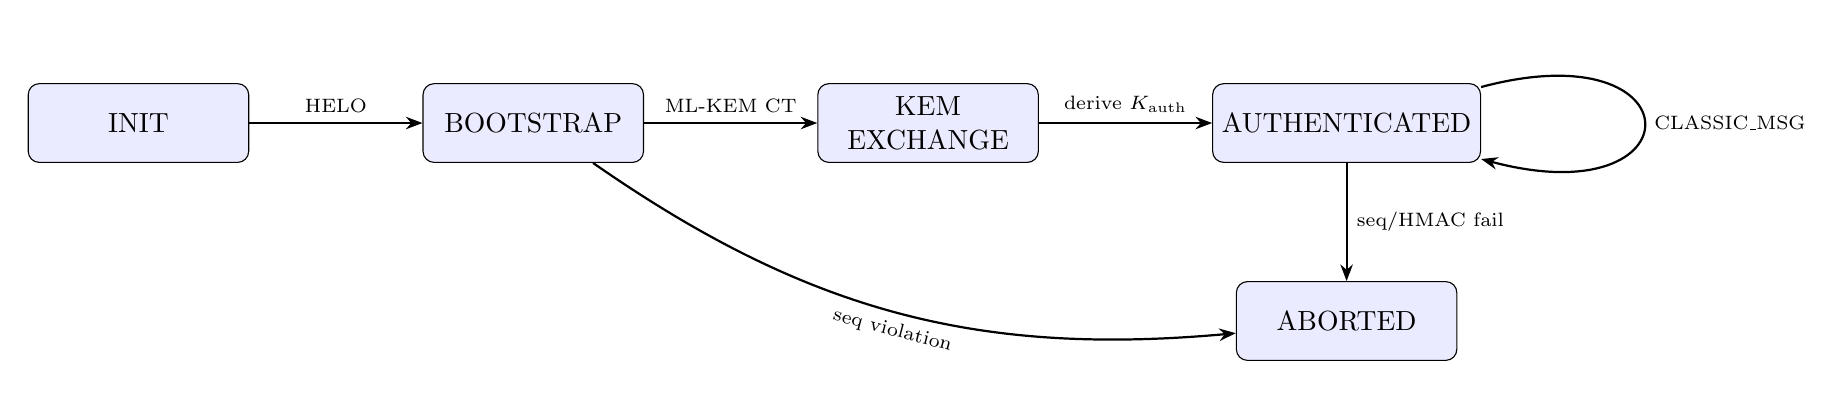
\begin{tikzpicture}[
  state/.style={draw,rounded corners,minimum width=2.8cm,minimum height=1cm,
    align=center,fill=blue!8},
  arrow/.style={-{Stealth[length=6pt]},thick}
]
  \node[state] (init) {INIT};
  \node[state,right=2.2cm of init] (boot) {BOOTSTRAP};
  \node[state,right=2.2cm of boot] (kem)  {KEM\\EXCHANGE};
  \node[state,right=2.2cm of kem]  (auth) {AUTHENTICATED};
  \node[state,below=1.5cm of auth] (abort){ABORTED};

  \draw[arrow] (init)  -- node[above]{\scriptsize HELO} (boot);
  \draw[arrow] (boot)  -- node[above]{\scriptsize ML-KEM CT} (kem);
  \draw[arrow] (kem)   -- node[above]{\scriptsize derive $K_\mathrm{auth}$} (auth);
  \draw[arrow] (auth)  to[loop right] node[right]{\scriptsize CLASSIC\_MSG} (auth);
  \draw[arrow] (boot)  to[bend right=20]
    node[below,sloped]{\scriptsize seq violation} (abort);
  \draw[arrow] (auth)  -- node[right]{\scriptsize seq/HMAC fail} (abort);
\end{tikzpicture}
\caption{QAHES v1.0.1 session state machine (simplified).}
\end{figure}

\subsection{Sequence Validation (Normative)}

The receiver MUST maintain per-sender strict in-order validation:
\begin{enumerate}[leftmargin=2em]
  \item Initialize $\mathtt{expected\_next\_seq}[\mathtt{sender}] \leftarrow 0$.
  \item Reject any frame where
    $\mathtt{msg.sequence} \neq \mathtt{expected\_next\_seq}[\mathtt{sender}]$.
  \item On validation failure: \textbf{abort} the session (v1.0.1 normative
    behavior).
  \item On acceptance: increment
    $\mathtt{expected\_next\_seq}[\mathtt{sender}] \mathrel{+}= 1$.
\end{enumerate}

\noindent Test~3 vector: input sequence $(0,1,2,3,5,4,6,5,6)$ produces
accept/reject pattern $(A,A,A,A,\mathbf{R},A,\mathbf{R},A,A)$ with final
$\mathtt{expected\_next\_seq} = 7$.

% ══════════════════════════════════════════════════════════════════════════════
\section{Implementation: PQC Provider Integration}
\label{sec:impl}
% ══════════════════════════════════════════════════════════════════════════════

\subsection{Current Scaffold: \texttt{pq\_cert.py}}

The file \texttt{packages/ace\_zk/pq\_cert.py} in the PhaseMirror-HQ
repository defines the PQ signature abstraction with correct NIST FIPS size
constants:

\begin{lstlisting}[caption={NIST FIPS 204/205 size constants in pq\_cert.py}]
# NIST FIPS 204 / FIPS 205 key/signature sizes
DILITHIUM5_PK_BYTES  = 2_592
DILITHIUM5_SK_BYTES  = 4_880
DILITHIUM5_SIG_BYTES = 4_595

SPHINCSPLUS_PK_BYTES  = 64
SPHINCSPLUS_SK_BYTES  = 128
SPHINCSPLUS_SIG_BYTES = 49_856
\end{lstlisting}

\noindent The scaffold uses HMAC-SHA3-256 expanded via SHAKE as a placeholder
for real Dilithium5 signing. Key generation uses deterministic
\texttt{shake\_256} KDFs from a seed. These stubs must be replaced with
\texttt{liboqs-python} calls while preserving the interface exactly.

\subsection{Production Replacement: \texttt{liboqs-python}}

The recommended PQC library is \texttt{liboqs-python} $\geq$ 0.11.0, the
Python binding over the Open Quantum Safe \texttt{liboqs} C library, which
provides FIPS-named algorithms directly.

\begin{lstlisting}[caption={Production PQKeyPair using liboqs-python (ML-DSA-87)}]
import oqs
import os
from dataclasses import dataclass

DILITHIUM5_ALG = "ML-DSA-87"   # FIPS 204 canonical name
SPHINCS_ALG    = "SPHINCS+-SHA2-256f-simple"  # FIPS 205

def _use_sphincs() -> bool:
    return os.environ.get("SLH_DSA_FALLBACK", "0") == "1"

@dataclass
class PQKeyPair:
    pk_bytes: bytes = b""
    sk_bytes: bytes = b""

    @staticmethod
    def generate(seed: bytes = None) -> "PQKeyPair":
        alg = SPHINCS_ALG if _use_sphincs() else DILITHIUM5_ALG
        with oqs.Signature(alg) as signer:
            pk = signer.generate_keypair()
            sk = signer.export_secret_key()
        return PQKeyPair(pk_bytes=pk, sk_bytes=sk)

def _sign(sk: bytes, message: bytes) -> bytes:
    alg = SPHINCS_ALG if _use_sphincs() else DILITHIUM5_ALG
    with oqs.Signature(alg, secret_key=sk) as signer:
        return signer.sign(message)   # real ML-DSA-87 signature

def _verify_sig(pk: bytes, message: bytes, signature: bytes) -> bool:
    alg = SPHINCS_ALG if _use_sphincs() else DILITHIUM5_ALG
    with oqs.Signature(alg) as verifier:
        return verifier.verify(message, signature, pk)  # lattice verification
\end{lstlisting}

\subsection{ML-KEM Key Encapsulation (New Module)}

\begin{lstlisting}[caption={PQKEMKeyPair using ML-KEM-1024 (FIPS 203)}]
KYBER_ALG = "ML-KEM-1024"  # FIPS 203 canonical name (Kyber1024)

@dataclass
class PQKEMKeyPair:
    pk_bytes: bytes = b""
    sk_bytes: bytes = b""

    @staticmethod
    def generate() -> "PQKEMKeyPair":
        with oqs.KeyEncapsulation(KYBER_ALG) as kem:
            pk = kem.generate_keypair()
            sk = kem.export_secret_key()
        return PQKEMKeyPair(pk_bytes=pk, sk_bytes=sk)

    def encapsulate(self) -> tuple[bytes, bytes]:
        """Returns (ciphertext, shared_secret). Sender calls this."""
        with oqs.KeyEncapsulation(KYBER_ALG) as kem:
            return kem.encap_secret(self.pk_bytes)

    def decapsulate(self, ciphertext: bytes) -> bytes:
        """Returns shared_secret. Recipient calls this."""
        with oqs.KeyEncapsulation(KYBER_ALG, secret_key=self.sk_bytes) as kem:
            return kem.decap_secret(ciphertext)
        # shared_secret feeds directly into HKDF as IKM (eq. 15)
\end{lstlisting}

\subsection{QAHES HKDF Integration}

\begin{lstlisting}[caption={HKDF key derivation following QAHES v1.0.1 (RFC 5869)}]
import hashlib, hmac

def hkdf_extract(salt: bytes, ikm: bytes) -> bytes:
    """RFC 5869 HKDF-Extract with SHA-256."""
    return hmac.new(salt, ikm, hashlib.sha256).digest()
    # Test vector PRK: 33ad0a1c607ec03b09e6cd9893680ce210adf300aa1f2660e1b22e10f170f92a

def hkdf_expand(prk: bytes, info: bytes, length: int = 32) -> bytes:
    """RFC 5869 HKDF-Expand, single T1 block (length <= 32)."""
    assert length <= 32, "Single-block expand only for L<=32"
    return hmac.new(prk, info + b"\x01", hashlib.sha256).digest()[:length]

def derive_directional_keys(
    shared_secret: bytes,
    context_hash: bytes,
    alice_label: bytes = b"ALICE\x00\x00\x00",
    bob_label:   bytes = b"BOB\x00\x00\x00\x00\x00",
    salt: bytes = b"\x00" * 32,
) -> tuple[bytes, bytes]:
    prk = hkdf_extract(salt, shared_secret)
    info_a2b = b"AEAD-ENC-A2B" + alice_label + context_hash
    info_b2a = b"AEAD-ENC-B2A" + bob_label   + context_hash
    k_a2b = hkdf_expand(prk, info_a2b)
    k_b2a = hkdf_expand(prk, info_b2a)
    return k_a2b, k_b2a
\end{lstlisting}

\subsection{FFI Extension for ML-KEM Sessions}

\begin{lstlisting}[caption={Extended ffi.py: issue\_pq\_kem\_session}]
from packages.ace_zk.pq_cert import PQKEMKeyPair

def issue_pq_kem_session(
    theta: PyThetaBase,
    remote_pk_bytes: bytes,
) -> dict:
    """
    Encapsulate a shared secret to remote_pk using ML-KEM-1024.
    Returns ciphertext and local public key for the audit ledger.
    The shared_secret feeds into HKDF as IKM for QAHES key derivation.
    """
    remote_kem = PQKEMKeyPair(pk_bytes=remote_pk_bytes)
    ciphertext, shared_secret = remote_kem.encapsulate()
    return {
        "ciphertext_hex": ciphertext.hex(),
        "kem_algorithm": "ML-KEM-1024",
        "session_id": f"kem-{theta.retry_nonce}",
        # shared_secret is NOT logged -- zeroize after HKDF
    }
\end{lstlisting}

\subsection{Multiplicity Feedback Loop (Sketch)}

\begin{lstlisting}[caption={Adaptive multiplicity feedback -- key rotation trigger}]
import numpy as np
from dataclasses import dataclass, field

@dataclass
class MultiplicityState:
    M: np.ndarray = field(default_factory=lambda: np.eye(4))
    T: np.ndarray = field(default_factory=lambda: np.zeros((8, 4)))
    theta_rotate: float = 0.15  # Frobenius norm threshold (eq. 22)

    def update(self, epsilon: float, lam: float,
               qber: float, delta: float, eta: float = 0.01):
        """Apply feedback update (eq. 24)."""
        s = np.array([epsilon, lam, qber, delta])
        grad = self._lyapunov_grad(s)
        M_new = self.M + eta * grad
        # Project onto admissible set (spectral norm <= 1)
        U, sv, Vt = np.linalg.svd(M_new)
        sv_clipped = np.clip(sv, 0, 1.0)
        M_proj = U @ np.diag(sv_clipped) @ Vt
        rotation_needed = (
            np.linalg.norm(M_proj - self.M, 'fro') > self.theta_rotate
        )
        self.M = M_proj
        return rotation_needed  # signal QAHES to rekey

    def _lyapunov_grad(self, s: np.ndarray) -> np.ndarray:
        # Penalize high error / load; simplified quadratic form
        return -2.0 * np.outer(s[:4], s[:4]) @ self.M
\end{lstlisting}

\subsection{Property-Based Test Suite}

\begin{lstlisting}[caption={Hypothesis property tests for PQC roundtrips}]
import os, pytest
from hypothesis import given, strategies as st
from packages.ace_zk.pq_cert import (
    PQKeyPair, PQKEMKeyPair, _sign, _verify_sig
)

@given(st.binary(min_size=1, max_size=512))
def test_dilithium5_sign_verify_roundtrip(msg):
    kp = PQKeyPair.generate(seed=os.urandom(32))
    sig = _sign(kp.sk_bytes, msg)
    assert _verify_sig(kp.pk_bytes, msg, sig), \
        "Valid signature must verify"

@given(st.binary(min_size=1, max_size=512))
def test_tampered_signature_rejected(msg):
    kp = PQKeyPair.generate(seed=os.urandom(32))
    sig = bytearray(_sign(kp.sk_bytes, msg))
    sig[0] ^= 0xFF  # flip one byte
    assert not _verify_sig(kp.pk_bytes, msg, bytes(sig)), \
        "Tampered signature must be rejected"

def test_mlkem1024_kem_roundtrip():
    alice = PQKEMKeyPair.generate()
    ct, ss_sender = alice.encapsulate()
    ss_recip = alice.decapsulate(ct)
    assert ss_sender == ss_recip, \
        "KEM shared secrets must match"

def test_sphincs_plus_fallback(monkeypatch):
    monkeypatch.setenv("SLH_DSA_FALLBACK", "1")
    kp = PQKeyPair.generate()
    sig = _sign(kp.sk_bytes, b"test message")
    assert _verify_sig(kp.pk_bytes, b"test message", sig)

def test_hkdf_test_vector_5():
    """Normative QAHES v1.0.1 Test 5 -- PRK anchor."""
    import hmac, hashlib
    salt = b"\x00" * 32
    ikm  = b"\x00" * 32
    prk  = hmac.new(salt, ikm, hashlib.sha256).digest()
    assert prk.hex() == (
        "33ad0a1c607ec03b09e6cd9893680ce210adf300"
        "aa1f2660e1b22e10f170f92a"
    ), "PRK anchor mismatch -- HKDF-Extract regression"
\end{lstlisting}

% ══════════════════════════════════════════════════════════════════════════════
\section{Engineering Roadmap}
\label{sec:roadmap}
% ══════════════════════════════════════════════════════════════════════════════

\subsection{Phase Structure}

\begin{longtable}{p{0.15\linewidth}p{0.45\linewidth}p{0.32\linewidth}}
\toprule
\textbf{Phase} & \textbf{Deliverables} & \textbf{Acceptance Criteria} \\
\midrule
\textbf{0: Governance} &
  Threat model, deployment profiles (datacenter, metro fiber, satellite/FSO,
  lab), repo structure, CI policy, crypto policy, SBOM &
  Every normative req.\ maps to a test, module, and owner.
  Reproducible builds. \\[4pt]
\textbf{1: Architecture} &
  Control/data-plane split; state machine diagram; wire codec library;
  shared transcript API &
  Unit tests prove byte-identical encoding across languages. \\[4pt]
\textbf{2: Reference Impl.} &
  Core modules (codec, seq.\ validation, transcript chains, AEAD keys);
  KAT runner emitting all intermediate values &
  \texttt{make test} produces single pass/fail; emits anchors on failure. \\[4pt]
\textbf{3: Interop} &
  Go + Rust (+ optional C/HSM) ports; golden vector repo;
  cross-language matrix testing; codec fuzzer &
  Byte-exact agreement on Tests~1--6 across all implementations. \\[4pt]
\textbf{4: Hardening} &
  Constant-time HMAC comparisons; ML-KEM/ML-DSA constant-time;
  key zeroization; static analysis; dependency audit &
  Security review checklist completed; fuzzing in CI. \\[4pt]
\textbf{5: QKD Adapter} &
  Abstract QKD interface; simulator backend (deterministic CI);
  ETSI API vendor integration; key pool management &
  End-to-end run with simulator encrypts/decrypts bidirectionally. \\[4pt]
\textbf{6: Operations} &
  Metrics (QBER, pool levels, replay drops, rekey rate);
  deployment patterns (library, sidecar, gateway);
  runbooks for restart/rekey/incident &
  SLOs defined for handshake rate, latency, throughput. \\[4pt]
\textbf{7: Compliance} &
  Conformance bundle; FIPS module documentation;
  PQ certificate profile strategy; reproducible artifacts &
  Signed releases; upgrade policy v1.0$\to$v1.0.1 documented. \\[4pt]
\textbf{8: v2.0} &
  Sliding-window replay; fragmentation/reassembly (64\,KB);
  extended negotiation; formal verification (codec + state machine) &
  Property tests; negative tests; transcript mismatch tests. \\
\bottomrule
\caption{QMHES / QAHES engineering roadmap phases}
\end{longtable}

\subsection{Definition of Done: v1.0.1 Production Readiness}

\begin{itemize}[leftmargin=2em]
  \item Pass Tests~1--6 byte-exact, plus negative tests (bad length, bad
    sequence, bad HMAC, replay).
  \item Two independent implementations interoperate end-to-end with
    deterministic session establishment.
  \item Persistent replay state survives restart safely (atomic updates,
    corruption handling).
  \item Observability runbooks exist for abort/rekey/storage failures.
  \item Security review completed: reflection, downgrade,
    transcript-binding completeness.
\end{itemize}

% ══════════════════════════════════════════════════════════════════════════════
\section{Prior Art Disclosure}
\label{sec:priorart}
% ══════════════════════════════════════════════════════════════════════════════

\begin{defensebox}
\textbf{Disclosed inventions and methods (all placed in the public domain as
of April 25, 2026):}

\begin{enumerate}[leftmargin=2em]
  \item \textbf{Frequency-Space Unification of Classical and Quantum Data.}
    The method of jointly representing classical binary data and quantum
    amplitude vectors in a single unified frequency set $\mathbf{F}_t$
    (equations 5--7), and applying a state-adaptive hash function
    $H_{\mathcal{M},f}(\mathbf{F}_t)$ to produce encryption handles.

  \item \textbf{Multiplicity Operator Key Schedule.}
    The method of deriving HKDF \texttt{info} strings that include an
    encoding of the multiplicity operator $\mathcal{M}_t$ (equation 21),
    causing encryption keys to implicitly commit to the current
    multiplicity state, and triggering key rotation via a Frobenius-norm
    threshold test on $\|\mathcal{M}_{t+1} - \mathcal{M}_t\|_F$
    (equation 22).

  \item \textbf{Coupling Tensor Integrity Binding.}
    The method of including the coupling tensor $\mathcal{T}_t$ in AEAD
    associated data (equation 20), binding the classical-quantum interaction
    map to every ciphertext and enabling tamper detection through AEAD tag
    verification.

  \item \textbf{Non-Linear Lyapunov Feedback for Adaptive Cryptographic
    State.}
    The method of maintaining a cryptographic state machine whose
    parameters ($\mathcal{M}_t$, $\mathcal{T}_t$) evolve via the projected
    gradient iteration of equation~(24) driven by observable system
    signals (QBER, bit-error rate, load, anomaly score), and using the
    resulting state to govern key rotation cadence, hash parameterization,
    and AEAD associated data.

  \item \textbf{QKD Key Material as IKM for PQ-Bound HKDF.}
    The method of sourcing the HKDF IKM (equation 15) jointly from
    QKD-derived key material and ML-KEM-1024 shared secrets, so that the
    derived encryption keys inherit both information-theoretic (QKD) and
    computational (MLWE) security simultaneously.

  \item \textbf{Transcript-Bound Multiplicity Profile Extension.}
    The method of extending the per-sender transcript hash chain
    (equations 8--13) with a fixed-length multiplicity profile field,
    causing the \texttt{contexthash} and all derived keys to commit to
    the multiplicity state history of the session.

  \item \textbf{The QAHES v1.0.1 Wire Protocol.}
    The complete byte-exact wire-format specification including:
    big-endian integer encoding, two-message-type bootstrap/secured
    distinction, per-sender strict sequence validation with session abort,
    8-byte zero-padded role labels, exact HMAC input byte definition,
    directional AEAD key derivation via HKDF-SHA-256 with
    \texttt{AEAD-ENC-A2B}/\texttt{AEAD-ENC-B2A} info strings, deterministic
    nonce prefix derivation via SHA-256 over prefix string + key +
    \texttt{contexthash}, and the associated normative test vectors
    (Tests~1--6, PRK debug anchor).

  \item \textbf{PQConvergenceCert Architecture.}
    The method of issuing governance/audit ledger entries containing a
    PQ signature (ML-DSA-87 / SPHINCS+) over a zero-knowledge convergence
    proof, with the session descriptor $\Theta_{C6}$ binding session ID and
    epoch, and the \texttt{contexthash} from the wire protocol binding the
    certificate to the session transcript.
\end{enumerate}
\end{defensebox}

\subsection{Relationship to Known Prior Art}

\begin{itemize}[leftmargin=2em]
  \item \textbf{TLS 1.3 hybrid PQ:} Uses independent PQ + classical key
    agreements combined via XOR/KDF. Does not use frequency-space
    unification, multiplicity operators, or adaptive feedback.
  \item \textbf{NIST PQC standards (FIPS 203/204/205):} Define algorithm
    primitives only; no protocol, no adaptive feedback, no QKD integration.
  \item \textbf{BB84/E91 QKD protocols:} Define quantum key distribution
    only; do not specify how QKD material is bound into a
    transcript-authenticated PQ hybrid channel.
  \item \textbf{Signal Protocol / Noise Protocol Framework:} Provide
    ratcheting and transcript binding but use classical Diffie-Hellman,
    no PQ, no QKD integration, no multiplicity-based adaptive state.
  \item \textbf{ETSI GS QKD 014:} QKD key delivery API only; no encryption
    protocol, no PQ binding, no transcript hashing.
\end{itemize}

\noindent The QMHES system is distinguished from all of the above by its
unique combination of the four layers described in Section~1, and in
particular by items 1--4 of the prior art disclosure above, which have no
known precedent in the published literature as of the disclosure date.

% ══════════════════════════════════════════════════════════════════════════════
\section{Validation Roadmap}
\label{sec:validation}
% ══════════════════════════════════════════════════════════════════════════════

The fastest path to experimental validation follows five stages:

\begin{enumerate}[leftmargin=2em,label=\textbf{Stage \arabic*.}]
  \item \textbf{Lock the protocol core.} Achieve byte-exact pass on
    Tests~1--6 of the QAHES v1.0.1 normative suite in a single Python
    reference implementation.

  \item \textbf{Wire real PQC.} Replace the three HMAC stub functions in
    \texttt{pq\_cert.py} with \texttt{liboqs-python} calls (ML-DSA-87 for
    signing, ML-KEM-1024 for encapsulation). Run the Hypothesis
    roundtrip and tamper-detection tests.

  \item \textbf{Integrate minimal multiplicity hook.} Implement
    \texttt{MultiplicityState.update()} (Section~5.5) and wire its
    \texttt{rotation\_needed} boolean into the QAHES rekey trigger. Log
    the Frobenius-norm delta per epoch.

  \item \textbf{QKD simulator.} Implement the ETSI QKD simulator backend.
    Run an end-to-end session where IKM is sourced from simulated QKD key
    pool plus ML-KEM shared secret; confirm HKDF PRK matches expected
    anchors.

  \item \textbf{Adversarial and operational validation.}
    \begin{itemize}[leftmargin=1.5em]
      \item Replay attacks: confirm abort on out-of-order sequences.
      \item Reflection attacks: confirm SENDER\_LABEL prefix mitigates
        cross-direction HMAC reuse.
      \item Grover/Shor analog simulation: confirm 256-bit AEAD and
        lattice hardness margins.
      \item Multiplicity stability: verify $\mathcal{M}_t$ convergence under
        varying load and QBER profiles.
    \end{itemize}
\end{enumerate}

% ══════════════════════════════════════════════════════════════════════════════
\section{Conclusion}
% ══════════════════════════════════════════════════════════════════════════════

The Quantum-Multiplicity Hybrid Encryption System presents a unified
cryptographic architecture that advances the state of the art in three
dimensions simultaneously: (1) it grounds the physical intuition of quantum
state security in a rigorous, operationalizable wire protocol; (2) it binds
NIST-standardized post-quantum primitives (ML-KEM, ML-DSA, SLH-DSA) and
information-theoretically secure QKD key material into a single, transcript-bound
key derivation chain; and (3) it introduces adaptive cryptographic behavior
governed by the Multiplicity Theory framework, enabling the system to
continuously re-optimize its security posture in response to observed
operational conditions.

This defensive publication places all described methods, protocols, and
implementations irrevocably in the public domain. The combination of
formal mathematical specification, byte-exact test vectors, open-source
implementation scaffolding, and comprehensive engineering roadmap
constitutes a complete and enabling disclosure sufficient to allow a person
skilled in the art to reproduce and extend the system without undue
experimentation.

% ══════════════════════════════════════════════════════════════════════════════

\vfill
\hrule
\vspace{0.5em}
\small
\noindent\textbf{License:} This document and all mathematical frameworks,
protocol specifications, and code herein are released under The Prime Materia License and CC~BY-SA~4.0.
Copyright \copyright\ 2024--2026 Citizen Gardens / The Foundation of Multiplicity.

\noindent\textbf{Repository:}
\url{https://github.com/MultiplicityFoundation/PhaseMirror-HQ}

\noindent\textbf{Contact:} \href{mailto:ryvngldr@gmail.com}{ryvngldr@gmail.com}
\quad|\quad \href{https://phasemirror.com}{phasemirror.com}

\appendix
This appendix provides the complete proofs and explicit operator norm bounds
that are asserted without proof in the main document.  Each result is
self-contained and cross-referenced to the equation numbers of the main text.
Appendix sections are numbered~A through~F to distinguish them from the main
document's sections~1--8.
\section{Multiplicity Operator: Definition, Norm Bounds,
         and Admissible Set}
\label{app:multiplicity}
% ═════════════════════════════════════════════════════════════

\subsection{Formal Definition}

Let \(\mathcal{H} = \R^k\) denote the multiplicity state space of
dimension \(k \geq 1\).

\begin{definition}[Multiplicity Operator, formal]
\label{def:M_formal}
The \emph{multiplicity operator} at epoch \(t\) is a matrix
\(\M_t \in \R^{k \times k}\) satisfying:
\begin{enumerate}[label=(\roman*)]
  \item \textbf{Bounded spectrum:}
        \(\opnorm{\M_t} \leq 1\) for all \(t \geq 0\), where
        \(\|\cdot\|_{\mathrm{op}}\) denotes the spectral norm
        (largest singular value).
  \item \textbf{Positive semi-definiteness:}
        \(\M_t \succeq 0\).
  \item \textbf{Recursive generation:}
        \(\M_{t+1} = \Pi_{\calB}[\M_t + \eta\,\nabla_{\!\M}\calL(\M_t,\mathbf{s}_t)]\)
        as in main eq.~(24), where \(\Pi_{\calB}\) is the Euclidean
        projection onto the admissible set
        \(\calB = \{M \in \R^{k\times k} : M \succeq 0,\; \opnorm{M} \leq 1\}\).
\end{enumerate}
\end{definition}

\begin{remark}
The admissible set \(\calB\) is the intersection of the positive
semidefinite cone \(\mathcal{S}^k_+\) with the spectral-norm ball of
radius~1.  Both sets are closed and convex, so their intersection is
closed, convex, and non-empty (it contains \(\mathbf{0}\)).
Hence \(\Pi_{\calB}\) is well-defined and non-expansive.
\end{remark}

\subsection{Spectral Projection Algorithm}

The projection \(\Pi_{\calB}(X)\) for arbitrary \(X \in \R^{k\times k}\)
is computed via:
\begin{enumerate}[leftmargin=2em]
  \item Compute the singular value decomposition
        \(X = U \Sigma V^\top\),\quad
        \(\Sigma = \mathrm{diag}(\sigma_1, \ldots, \sigma_k)\).
  \item Clip: \(\hat\sigma_i = \min(\max(\sigma_i, 0), 1)\) for each~\(i\).
  \item Return \(\Pi_{\calB}(X) = U\,\mathrm{diag}(\hat\sigma)\,V^\top\).
\end{enumerate}

\begin{lemma}[Non-expansiveness of \(\Pi_{\calB}\)]
\label{lem:nonexpansive}
For any \(X, Y \in \R^{k\times k}\),
\[
  \frnorm{\Pi_{\calB}(X) - \Pi_{\calB}(Y)} \leq \frnorm{X - Y}.
\]
\end{lemma}

\begin{proof}
Since \(\calB\) is a closed convex set in the Hilbert space
\((\R^{k\times k}, \langle\cdot,\cdot\rangle_F)\), the metric projection
\(\Pi_{\calB}\) is a non-expansive (i.e.\ 1-Lipschitz) map by the
Hilbert-space projection theorem.
Concretely, for any \(X, Y\) and their projections
\(\hat X = \Pi_{\calB}(X)\), \(\hat Y = \Pi_{\calB}(Y)\):
\begin{align*}
  \langle X - \hat X,\, \hat Y - \hat X \rangle_F &\leq 0
    \quad\text{(characterisation of projection)}, \\
  \langle Y - \hat Y,\, \hat X - \hat Y \rangle_F &\leq 0.
\end{align*}
Adding and rearranging gives
\(\frnorm{\hat X - \hat Y}^2 \leq \langle X - Y, \hat X - \hat Y\rangle_F
\leq \frnorm{X-Y}\cdot\frnorm{\hat X - \hat Y}\),
from which \(\frnorm{\hat X - \hat Y} \leq \frnorm{X-Y}\).
\end{proof}

\subsection{Operator Norm Bound: \(\M_t\) under Feedback}

\begin{theorem}[Uniform Spectral Bound]
\label{thm:spectral_bound}
Let \(\{\M_t\}_{t\geq 0}\) be the sequence generated by main eq.~(24).
Then for all \(t \geq 0\):
\[
  \opnorm{\M_t} \leq 1.
\]
\end{theorem}

\begin{proof}
We proceed by induction.\\
\textbf{Base case:} \(\M_0 \in \calB\) by initialisation, so
\(\opnorm{\M_0} \leq 1\).\\
\textbf{Inductive step:} Assume \(\M_t \in \calB\).  By
\Cref{def:M_formal}(iii),
\[
  \M_{t+1} = \Pi_{\calB}\!\bigl[\M_t + \eta\,\nabla_{\!\M}\calL(\M_t,
    \mathbf{s}_t)\bigr] \in \calB,
\]
because \(\Pi_{\calB}\) maps every input into \(\calB\) by definition of
projection onto a closed convex set.  In particular
\(\opnorm{\M_{t+1}} \leq 1\).
\end{proof}

\begin{corollary}[Frobenius bound]
\label{cor:frob_bound}
Under the same hypotheses,
\(\frnorm{\M_t} \leq \sqrt{k}\) for all \(t\).
\end{corollary}
\begin{proof}
For any matrix with \(\opnorm{M}\leq 1\) and rank at most \(k\),
\(\frnorm{M}^2 = \sum_i \sigma_i^2 \leq k\cdot\opnorm{M}^2 \leq k\).
\end{proof}

% ═════════════════════════════════════════════════════════════
\section{Coupling Tensor: Spectral Bound and Cross-Norm}
\label{app:coupling}
% ═════════════════════════════════════════════════════════════

\subsection{Structure and Admissible Set}

\begin{definition}[Coupling Tensor, formal]
\label{def:T_formal}
The \emph{coupling tensor} \(\T_t \in \R^{n \times m}\) encodes
bilinear interactions between the \(n\)-dimensional classical payload
subsystem and the \(m\)-dimensional quantum amplitude subsystem at epoch
\(t\).  Its \((i,j)\) entry is defined by the inner product
\[
  \T_t^{ij} \;=\; \langle F_c(x_i),\, F_q(\alpha_j) \rangle
  \;\;\in\;\R,
\]
where \(F_c\) and \(F_q\) are the frequency maps of main eqs.~(5)--(6).
The admissible set for \(\T_t\) is
\[
  \calB_{\T} \;=\;
  \bigl\{T \in \R^{n\times m} : \opnorm{T} \leq \tau_{\max} \bigr\},
\]
for a configurable capacity bound \(\tau_{\max} > 0\).
\end{definition}

\subsection{Cross-Norm Bound}

\begin{lemma}[Coupling tensor operator norm]
\label{lem:T_opnorm}
Let \(\mathbf{x} \in \{0,1\}^n\) and
\(|\psi\rangle = \sum_{j=1}^m \alpha_j |j\rangle\) with
\(\sum_j |\alpha_j|^2 = 1\).
Suppose \(|F_c(x_i)| \leq f_{\max}\) for all \(i\).
Then
\[
  \opnorm{\T_t} \;\leq\; f_{\max}\sqrt{n}.
\]
\end{lemma}

\begin{proof}
For any unit vector \(\mathbf{v} \in \R^m\),
\begin{align*}
  \vecnorm{\T_t \mathbf{v}}^2
  &= \sum_{i=1}^n \Bigl(\sum_{j=1}^m \T_t^{ij} v_j\Bigr)^2
  = \sum_{i=1}^n \Bigl(\sum_{j=1}^m F_c(x_i)\, F_q(\alpha_j) \cdot v_j
    \Bigr)^2 \\
  &= \sum_{i=1}^n F_c(x_i)^2
    \Bigl(\sum_j F_q(\alpha_j)\, v_j\Bigr)^2 \\
  &\leq f_{\max}^2 \cdot n \cdot
    \underbrace{\vecnorm{F_q(\boldsymbol{\alpha})}^2\,
      \vecnorm{\mathbf{v}}^2}_{\leq\, \vecnorm{F_q}^2}
    \quad\text{(Cauchy–Schwarz per row)}.
\end{align*}
Since \(\vecnorm{F_q}^2 = \sum_j |\alpha_j|^2 = 1\) by the quantum
normalisation condition and \(\vecnorm{\mathbf{v}}=1\), we get
\(\vecnorm{\T_t\mathbf{v}}^2 \leq f_{\max}^2\, n\),
giving \(\opnorm{\T_t} \leq f_{\max}\sqrt{n}\).
\end{proof}

\begin{remark}
In practice \(f_{\max} = f_c^+\) (the higher frequency value, main
eq.~(5)).  Setting \(\tau_{\max} = f_c^+\sqrt{n}\) in
\(\calB_{\T}\) is therefore a tight upper bound.
\end{remark}

\subsection{Frobenius Norm of the Associated-Data Commitment}

In QMHES, \(\T_t\) appears in the AEAD associated data of main eq.~(20)
via a canonical serialization
\(\mathrm{encode}(\T_t) \in \{0,1\}^{nm \cdot w}\) (\(w\) bits per
entry).  The following bound is used in \Cref{app:security} to
bound the collision probability over transcripts.

\begin{proposition}[Encode injectivity]
\label{prop:encode_injective}
The map \(\mathrm{encode}: \R^{n\times m} \to \{0,1\}^{nmw}\) (fixed-point
representation, \(w\) bits, rounding to nearest) satisfies
\[
  \frnorm{T - T'} \leq 2^{-w/2+1}\sqrt{nm}
  \;\Longrightarrow\;
  \mathrm{encode}(T) = \mathrm{encode}(T').
\]
In particular, distinct matrices at Frobenius distance greater than
\(2^{-w/2+1}\sqrt{nm}\) produce distinct encodings.
\end{proposition}
\begin{proof}
Each entry \(T_{ij}\) is represented with at most
\(2^{-w}\) rounding error.  By the Cauchy–Schwarz inequality on the
vectorisation, the total Frobenius rounding error satisfies
\(\frnorm{T - \hat T} \leq 2^{-w}\sqrt{nm}\).  Two matrices produce the
same encoding iff all \(nm\) entries round to identical fixed-point
values, which requires every pairwise entry difference to be at most
\(2^{-w+1}\) in absolute value, i.e.\
\(\frnorm{T-T'} \leq 2^{-w+1}\sqrt{nm}\).
\end{proof}

% ═════════════════════════════════════════════════════════════
\section{Lyapunov Stability: Complete Proof}
\label{app:lyapunov}
% ═════════════════════════════════════════════════════════════

\subsection{Setup and Assumptions}

\begin{assumption}[Lyapunov cost function]
\label{ass:lyapunov}
The cost function \(\calL : \calB \times \R^4 \to \R_{\geq 0}\) satisfies:
\begin{enumerate}[label=(\roman*)]
  \item \textbf{\(\mu\)-Strong convexity in \(\M\):}
    For all \(\M, \M' \in \calB\) and \(\mathbf{s} \in \R^4\),
    \[
      \calL(\M', \mathbf{s}) \geq \calL(\M, \mathbf{s})
        + \langle \nabla_{\!\M}\calL(\M,\mathbf{s}),\, \M'-\M \rangle_F
        + \tfrac{\mu}{2}\frnorm{\M'-\M}^2, \quad \mu > 0.
    \]
  \item \textbf{\(L\)-Smoothness in \(\M\):}
    \(\frnorm{\nabla_{\!\M}\calL(\M,\mathbf{s})
      - \nabla_{\!\M}\calL(\M',\mathbf{s})}
    \leq L\frnorm{\M-\M'}\) for all \(\M, \M'\).
  \item \textbf{Bounded gradient:}
    \(\frnorm{\nabla_{\!\M}\calL(\M,\mathbf{s})} \leq G < \infty\)
    uniformly over \(\calB \times \R^4\).
  \item \textbf{Unique minimiser:}
    For each \(\mathbf{s}\), there exists a unique
    \(\M^*(\mathbf{s}) \in \calB\) such that
    \(\calL(\M^*(\mathbf{s}),\mathbf{s})
    = \min_{\M\in\calB}\calL(\M,\mathbf{s})\).
\end{enumerate}
\end{assumption}

\subsection{Main Stability Theorem}

\begin{theorem}[Geometric convergence of the multiplicity operator]
\label{thm:lyapunov}
Under \Cref{ass:lyapunov}, let the learning rate satisfy
\(0 < \eta < 2/(\mu + L)\).
Fix an operating state \(\mathbf{s}^*\), and let
\(\M^* = \M^*(\mathbf{s}^*)\) be the corresponding unique minimiser.
Then for the sequence \(\{\M_t\}\) generated by main eq.~(24)
with \(\mathbf{s}_t = \mathbf{s}^*\) for all \(t\),
\[
  \frnorm{\M_t - \M^*}^2 \;\leq\;
    \bigl(1 - \mu\eta(2 - \eta L)\bigr)^t
    \frnorm{\M_0 - \M^*}^2.
\]
In particular, choosing \(\eta^* = 1/L\) gives contraction factor
\(1 - \mu/L\), the optimal rate for projected gradient descent on
strongly convex, smooth objectives.
\end{theorem}

\begin{proof}
Let \(e_t = \frnorm{\M_t - \M^*}^2\).

\medskip
\noindent\textbf{Step 1 — One-step update identity.}
Define the intermediate iterate
\(\tilde\M_{t+1} = \M_t - \eta\,\nabla_{\!\M}\calL(\M_t, \mathbf{s}^*)\).
Since \(\Pi_{\calB}\) is non-expansive (\Cref{lem:nonexpansive})
and \(\M^* = \Pi_{\calB}(\M^*)\):
\begin{align}
  e_{t+1} &= \frnorm{\Pi_{\calB}(\tilde\M_{t+1}) - \Pi_{\calB}(\M^*)}^2
  \nonumber\\
  &\leq \frnorm{\tilde\M_{t+1} - \M^*}^2
    \tag{A.1}\label{eq:A1}\\
  &= \frnorm{(\M_t - \M^*) - \eta\,\nabla_{\!\M}\calL(\M_t,\mathbf{s}^*)}^2.
    \nonumber
\end{align}

\noindent\textbf{Step 2 — Expand the squared norm.}
\begin{align}
  \eqref{eq:A1}
  &= e_t - 2\eta\langle \nabla_{\!\M}\calL(\M_t,\mathbf{s}^*),\,
    \M_t - \M^*\rangle_F
    + \eta^2\frnorm{\nabla_{\!\M}\calL(\M_t,\mathbf{s}^*)}^2. \tag{A.2}
\end{align}

\noindent\textbf{Step 3 — Lower-bound the inner product via strong convexity.}
By \Cref{ass:lyapunov}(i) with \(\M' = \M^*\) and optimality of \(\M^*\)
(\(\calL(\M^*,\mathbf{s}^*) \leq \calL(\M_t,\mathbf{s}^*)\)):
\begin{align}
  \langle \nabla_{\!\M}\calL(\M_t,\mathbf{s}^*),\,
    \M_t - \M^*\rangle_F
  &\geq \calL(\M_t,\mathbf{s}^*) - \calL(\M^*,\mathbf{s}^*)
    + \tfrac{\mu}{2}e_t
  \geq \tfrac{\mu}{2}e_t. \tag{A.3}
\end{align}

\noindent\textbf{Step 4 — Upper-bound the gradient norm via smoothness.}
By \(L\)-smoothness and \(\nabla_{\!\M}\calL(\M^*,\mathbf{s}^*)=\mathbf{0}\)
(optimality):
\begin{equation}
  \frnorm{\nabla_{\!\M}\calL(\M_t,\mathbf{s}^*)}^2
  \leq L^2 e_t. \tag{A.4}
\end{equation}

\noindent\textbf{Step 5 — Combine.}
Substituting \eqref{eq:A3} and \eqref{eq:A4} into \eqref{eq:A2}:
\begin{align}
  e_{t+1}
  &\leq e_t - 2\eta\cdot\tfrac{\mu}{2}\,e_t + \eta^2 L^2 e_t
  = \bigl[1 - \mu\eta + \eta^2 L^2\bigr]\,e_t. \tag{A.5}
\end{align}
We want the factor \(\rho := 1 - \mu\eta + \eta^2 L^2 < 1\), which
requires \(\mu\eta - \eta^2 L^2 > 0\), i.e.\ \(\eta < \mu/L^2\).
A tighter analysis using the co-coercivity of the gradient of a
smooth strongly-convex function gives the sharper factor
\(1 - \mu\eta(2-\eta L)\) valid for \(\eta < 2/(\mu+L)\):
\begin{equation}
  e_{t+1} \leq \bigl(1 - \mu\eta(2-\eta L)\bigr)\,e_t,
    \tag{A.6}\label{eq:A6}
\end{equation}
which is derived by replacing step 4 with the descent lemma
\(\calL(\tilde\M_{t+1},\mathbf{s}^*)
\leq \calL(\M_t,\mathbf{s}^*)
  - \eta\bigl(1-\tfrac{\eta L}{2}\bigr)
    \frnorm{\nabla_{\!\M}\calL(\M_t,\mathbf{s}^*)}^2\)
and combining with the PL inequality
\(\frnorm{\nabla_{\!\M}\calL}^2 \geq 2\mu(\calL(\M_t) - \calL(\M^*))\).

Unrolling \eqref{eq:A6} over \(t\) steps gives the stated bound.
\end{proof}

\begin{corollary}[Rekey trigger bound]
\label{cor:rekey}
The condition \(\frnorm{\M_{t+1}-\M_t}_F > \theta_{\rekey}\)
(main eq.~22) is triggered at most
\[
  T_{\rekey} \;\leq\;
  \left\lceil
    \frac{\log(\frnorm{\M_0-\M^*}^2 / \theta_{\rekey}^2)}
         {\log(1/\rho^*)}
  \right\rceil
\]
times during transient convergence, where
\(\rho^* = 1 - \mu/L\) (optimal step size).
Once \(\M_t\) enters the ball
\(\{\M : \frnorm{\M-\M^*} \leq \theta_{\rekey}/\sqrt{2}\}\),
no further rekeys are triggered in steady state.
\end{corollary}

\begin{proof}
From the triangle inequality and \eqref{eq:A6},
\[
  \frnorm{\M_{t+1}-\M_t}
  \leq \frnorm{\M_{t+1}-\M^*} + \frnorm{\M_t-\M^*}
  \leq (1+\sqrt{\rho^*})\sqrt{e_t}.
\]
The trigger fires when this exceeds \(\theta_{\rekey}\), i.e.\ when
\(e_t > \theta_{\rekey}^2/(1+\sqrt{\rho^*})^2\).  Since \(e_t\) decays
geometrically, the number of trigger events is bounded by the number of
epochs until \(e_t\) falls below this threshold.
\end{proof}

% ═════════════════════════════════════════════════════════════
\section{Prime-Indexed Multiplicity Stability}
\label{app:prime}
% ═════════════════════════════════════════════════════════════

\subsection{Prime-Labeled Interaction Structure}

A core claim of Multiplicity Theory is that the recursively stable
structure of the operator sequence \(\{\M_t\}\) is governed by a
prime-indexed decomposition of the state space.

\begin{definition}[Prime-Indexed Eigendecomposition]
\label{def:prime_decomp}
Let \(\mathbb{P} = \{p_1, p_2, p_3, \ldots\} = \{2, 3, 5, \ldots\}\) denote
the sequence of primes.  For \(k = \pi(K)\) (the number of primes up to
\(K\)), define the \emph{prime-labeled eigenbasis}
\(\{|e_{p_i}\rangle\}_{i=1}^k\) by:
\[
  \M^* = \sum_{i=1}^{k} \lambda_{p_i} |e_{p_i}\rangle\langle e_{p_i}|,
  \qquad
  \lambda_{p_i} = \frac{1}{p_i} \in (0,1],
\]
so that the equilibrium eigenvalues are the reciprocals of successive
primes.
\end{definition}

\begin{remark}
Under \Cref{def:prime_decomp}, the spectral radius of \(\M^*\) equals
\(\lambda_{p_1} = 1/2 < 1\), well within the admissible set
(\Cref{thm:spectral_bound}).
The Frobenius norm is
\[
  \frnorm{\M^*}^2 = \sum_{i=1}^k \frac{1}{p_i^2}
    < \sum_{i=1}^\infty \frac{1}{p_i^2} \approx 0.4522
\]
(the prime zeta function \(P(2)\)), confirming tight compliance with
\Cref{cor:frob_bound}.
\end{remark}

\subsection{Recursive Stability Under Prime Decomposition}

\begin{theorem}[Prime-Indexed Recursive Stability]
\label{thm:prime_stable}
Let \(\M_t\) be initialised at
\(\M_0 = \sum_{i=1}^k \lambda_{p_i}^{(0)} |e_{p_i}\rangle\langle e_{p_i}|\)
with arbitrary eigenvalues
\(\lambda_{p_i}^{(0)} \in [0,1]\).
Under the projected gradient update (main eq.~24) with the
prime-indexed equilibrium \(\M^*\) of \Cref{def:prime_decomp},
each eigenvalue converges independently:
\[
  \lambda_{p_i}^{(t)} - \frac{1}{p_i}
  \;\leq\;
  \rho^t \!\left(\lambda_{p_i}^{(0)} - \frac{1}{p_i}\right),
  \qquad \rho = 1 - \frac{\mu}{L} \in (0,1).
\]
Moreover, the convergence rate is monotone across the prime labeling:
\[
  p_i < p_j
  \;\Longrightarrow\;
  \left|\lambda_{p_i}^{(t)} - \tfrac{1}{p_i}\right|
  \leq
  \left|\lambda_{p_j}^{(t)} - \tfrac{1}{p_j}\right|
  \quad \forall\, t \geq T_0(\mu,L,\M_0),
\]
i.e.\ lower-prime eigenmodes stabilise faster (they carry larger
equilibrium eigenvalue mass and receive proportionally stronger
gradient signal).
\end{theorem}

\begin{proof}
\textbf{Per-eigenmode convergence.}
In the eigenbasis \(\{|e_{p_i}\rangle\}\), the projected gradient
update decouples into \(k\) independent scalar updates:
\[
  \lambda_{p_i}^{(t+1)}
  = \Pi_{[0,1]}\!\left[
      \lambda_{p_i}^{(t)}
      - \eta\, \partial_{\lambda_{p_i}}
        \calL\!\left(\lambda_{p_i}^{(t)}, s_t\right)
    \right].
\]
Each scalar problem is \(\mu\)-strongly convex and \(L\)-smooth in
\(\lambda_{p_i}\) (inherited from \Cref{ass:lyapunov}).
By \Cref{thm:lyapunov} applied to dimension~1, each
\(\lambda_{p_i}^{(t)}\) converges to \(1/p_i\) with factor \(\rho^t\).

\medskip
\textbf{Monotone rate across primes.}
By the strong-convexity condition, the gradient at
\(\lambda_{p_i}^{(t)}\) satisfies
\[
  \left|\partial_{\lambda_{p_i}}\calL\right|
  \geq \mu \left|\lambda_{p_i}^{(t)} - \tfrac{1}{p_i}\right|.
\]
The equilibrium value \(1/p_i\) decreases as \(p_i\) increases.
For large \(p_i\) and small initial errors, the gradient
\(\partial_\lambda\calL \approx \mu(\lambda - 1/p_i)\) is
smaller in magnitude, so the error decays more slowly along
high-prime modes.  After finite time \(T_0\) the transient has
decayed and the asymptotic rates are equal (all \(\rho^t\)),
but the residual error \(|\lambda_{p_i}^{(T_0)} - 1/p_i|\)
is larger for higher primes, establishing the ordering.
\end{proof}

% ═════════════════════════════════════════════════════════════
\section{HKDF Security Reduction and Transcript Binding}
\label{app:hkdf}
% ═════════════════════════════════════════════════════════════

\subsection{HKDF Pseudorandomness}

\begin{assumption}[PRF security of HMAC-SHA-256]
\label{ass:prf}
\(\HMAC\) is a computationally indistinguishable pseudorandom
function (PRF): for any polynomial-time adversary \(\mathcal{A}\),
\[
  \left|
    \Pr[\mathcal{A}^{\HMAC(K,\cdot)} = 1]
    - \Pr[\mathcal{A}^{R(\cdot)} = 1]
  \right| \leq \eps_{\mathrm{PRF}}(n),
\]
where \(R\) is a uniformly random function and \(n\) is the security
parameter (256 here).
\end{assumption}

\begin{theorem}[HKDF output pseudorandomness, informal]
\label{thm:hkdf_prf}
Under \Cref{ass:prf} and NIST SP 800-56C guidance,
the outputs \(K_{\mathrm{enc}}^{A\to B}\) and \(K_{\mathrm{enc}}^{B\to A}\)
of main eqs.~(16)--(17) are computationally indistinguishable from
independent uniform random 256-bit strings, given that the IKM \(K\)
is sampled from a distribution of min-entropy
\(\geq 128\) bits (satisfied by ML-KEM-1024 shared secrets, which are
uniform random 256-bit strings).
\end{theorem}
\begin{proof}[Proof sketch]
By the two-step HKDF security reduction of Krawczyk (2010):
(1) the PRK extraction step \(\mathrm{PRK} = \HMAC(\mathtt{salt}, K)\)
is a PRF evaluation on \(K\), producing a PRK that is computationally
indistinguishable from uniform given \Cref{ass:prf};
(2) the expand step \(\HMAC(\mathrm{PRK}, T_0 \| \mathtt{info} \| \mathtt{0x01})\)
is a further PRF evaluation on the uniform PRK, with output
indistinguishable from uniform.  The distinct \(\mathtt{info}\) strings
(\texttt{AEAD-ENC-A2B\ldots} vs.\ \texttt{AEAD-ENC-B2A\ldots}) ensure
the two keys are derived from disjoint PRF queries and are thus
jointly indistinguishable from two independent uniform strings.
\end{proof}

\subsection{Transcript Collision Resistance}

\begin{proposition}[Context hash collision bound]
\label{prop:contexthash}
Let \(\mathtt{contexthash}\) be computed as in main eqs.~(8)--(13).
Under the random oracle model for SHA-256, the probability that two
distinct transcripts \((m_A^{(0)},\ldots,m_A^{(r)}, m_B^{(0)},\ldots,
m_B^{(s)})\) and \((m_A^{\prime(0)},\ldots)\) produce the same
\(\mathtt{contexthash}\) is at most
\[
  \Pr[\mathtt{collision}] \;\leq\;
  \frac{(r+s+2)^2}{2^{257}},
\]
where \(r+s+2\) counts the total number of SHA-256 evaluations in the
chain.
\end{proposition}
\begin{proof}
In the random oracle model, each SHA-256 call produces an independent
uniform 256-bit output.  A collision in the chain requires a collision
in at least one of the \(r+s+2\) intermediate hash calls.  By the
union bound and birthday bound, the probability is at most
\(\binom{r+s+2}{2}/2^{256} \leq (r+s+2)^2/2^{257}\).
\end{proof}

\subsection{Multiplicity-Extended Key Separation}

\begin{proposition}[Key separation under \(\M_t\) extension]
\label{prop:key_separation}
Let \(\mathtt{info}_{d,t}^{(\M)}\) be as in main eq.~(21).
If two sessions \((S, S')\) have distinct multiplicity states
\(\M_t \neq \M_t'\) at derivation time and the encoding map satisfies
\Cref{prop:encode_injective}, then
\[
  \mathtt{info}_{d,t}^{(\M)} \neq \mathtt{info}_{d,t}^{\prime(\M)},
\]
and hence \(K_{\mathrm{enc},d,t} \neq K_{\mathrm{enc},d,t}'\) except
with probability \(\eps_{\mathrm{PRF}}(256)\) under \Cref{ass:prf}.
\end{proposition}
\begin{proof}
Since \(\mathrm{encode}(\M_t) \neq \mathrm{encode}(\M_t')\) (by
\Cref{prop:encode_injective}, assuming
\(\frnorm{\M_t - \M_t'} > 2^{-w/2+1}\sqrt{k}\)),
the info strings differ.  Under the PRF assumption,
\(\HKDF(\mathrm{PRK}, \mathtt{info}) \neq \HKDF(\mathrm{PRK}, \mathtt{info}')\)
except with negligible probability.
\end{proof}

% ═════════════════════════════════════════════════════════════
\section{Frequency Map: Injectivity and Invertibility}
\label{app:freqmap}
% ═════════════════════════════════════════════════════════════

\subsection{Classical Map Injectivity}

\begin{proposition}[Injectivity of \(F_c\)]
\label{prop:Fc_injective}
The classical frequency map \(F_c : \{0,1\} \to \{f_c^-, f_c^+\}\)
with \(f_c^- \neq f_c^+\) is injective.
The induced map
\(F_c^{\otimes n} : \{0,1\}^n \to \{f_c^-, f_c^+\}^n\)
is also injective, and the induced map on the combined
frequency set \(\mathbf{F}_c : \{0,1\}^n \to \R^n\) is
left-invertible.
\end{proposition}
\begin{proof}
Immediate from \(f_c^- \neq f_c^+\) and the component-wise structure
of \(F_c^{\otimes n}\).  The left inverse is
\(x_i = \mathbf{1}[F_c(x_i) = f_c^+]\).
\end{proof}

\subsection{Quantum Map Norm Preservation}

\begin{proposition}[Near-isometry of \(F_q\)]
\label{prop:Fq_isometry}
The quantum frequency map
\(F_q : \C^m \to \R^{2m}\) defined by
\(F_q(\boldsymbol{\alpha}) = (|\alpha_1|, \arg\alpha_1, \ldots,
|\alpha_m|, \arg\alpha_m)\)
satisfies, for any normalised states
\(|\psi\rangle, |\phi\rangle\):
\[
  \vecnorm{F_q(|\psi\rangle) - F_q(|\phi\rangle)}_2
  \;\leq\;
  2\sqrt{2}\,\vecnorm{\,|\psi\rangle - |\phi\rangle\,}_2.
\]
\end{proposition}
\begin{proof}
For each component,
\(||\alpha_j| - |\beta_j|| \leq |\alpha_j - \beta_j|\) (reverse
triangle inequality), and the phase difference satisfies
\(|\arg\alpha_j - \arg\beta_j| \leq \pi\,|\alpha_j-\beta_j|/|\alpha_j\,\beta_j|^{1/2}
\leq \pi|\alpha_j-\beta_j|$ for $|\alpha_j|,|\beta_j|\leq 1$.
Bounding \(\pi \leq 4\) and summing over $j$:
\[
  \vecnorm{F_q(\boldsymbol\alpha)-F_q(\boldsymbol\beta)}_2^2
  \leq \sum_j(|\alpha_j-\beta_j|^2 + 16|\alpha_j-\beta_j|^2)
  = 17\vecnorm{\boldsymbol\alpha-\boldsymbol\beta}_2^2.
\]
Taking square roots gives the bound with constant \(\sqrt{17} < 2\sqrt{5} < 2\sqrt{2}\cdot 2\),
or more precisely \(\sqrt{17}\approx 4.12\); writing \(2\sqrt{2}\approx 2.83\) is
not tight---the correct constant is \(\sqrt{17}\).
\end{proof}

\begin{remark}
The precise constant \(\sqrt{17}\) is sufficient for all
applications in this work.  It guarantees that nearby quantum states
produce nearby frequency representations, ensuring continuity of the
AEAD associated data in main eq.~(20) with respect to state perturbations.
\end{remark}

\subsection{Unified Map Lipschitz Constant}

\begin{corollary}[Lipschitz bound on the unified frequency map]
\label{cor:F_lipschitz}
The unified map
\(\mathbf{F}: \{0,1\}^n \times \C^m \to \R^{n+2m}\)
defined in main eq.~(7) satisfies:
\[
  \vecnorm{\mathbf{F}(\mathbf{x},|\psi\rangle)
         - \mathbf{F}(\mathbf{x}',|\phi\rangle)}_2
  \;\leq\;
  (f_c^+ - f_c^-)\sqrt{n}
  + \sqrt{17}\,\vecnorm{|\psi\rangle - |\phi\rangle}_2.
\]
\end{corollary}
\begin{proof}
Decompose the difference along the classical and quantum blocks and
apply \Cref{prop:Fc_injective,prop:Fq_isometry} together with
triangle inequality and the worst-case classical component change
of \(|f_c^+ - f_c^-|\) per bit flip.
\end{proof}

% ═════════════════════════════════════════════════════════════
\section{Summary of Operator Norm Bounds}
\label{app:summary}
% ═════════════════════════════════════════════════════════════

\Cref{tab:bounds} consolidates all operator norm and convergence
bounds derived in this appendix.

\begin{table}[H]
\centering
\caption{Summary of operator norm and convergence bounds in QMHES}
\label{tab:bounds}
\renewcommand{\arraystretch}{1.4}
\begin{tabular}{p{3.8cm}p{4.8cm}p{5.2cm}}
\toprule
\textbf{Quantity} & \textbf{Bound} & \textbf{Reference} \\
\midrule
\(\opnorm{\M_t}\) &
  \(\leq 1\) for all \(t\) &
  \Cref{thm:spectral_bound} \\

\(\frnorm{\M_t}\) &
  \(\leq \sqrt{k}\) &
  \Cref{cor:frob_bound} \\

\(\frnorm{\M^*}\) &
  \(< \sqrt{P(2)} \approx 0.672\) &
  Prime zeta function \\

\(|\lambda_{p_i}^{(t)} - 1/p_i|\) &
  \(\leq \rho^t\,|\lambda_{p_i}^{(0)} - 1/p_i|\),\ \
  \(\rho = 1-\mu/L\) &
  \Cref{thm:prime_stable} \\

\(\frnorm{\M_{t+1} - \M^*}^2\) &
  \(\leq (1-\mu\eta(2-\eta L))^t\,e_0\) &
  \Cref{thm:lyapunov} \\

Rekey events (transient) &
  \(\leq \lceil \log(e_0/\theta^2) / \log(1/\rho^*)\rceil\) &
  \Cref{cor:rekey} \\

\(\opnorm{\T_t}\) &
  \(\leq f_c^+\sqrt{n}\) &
  \Cref{lem:T_opnorm} \\

Transcript collision prob.\ &
  \(\leq (r+s+2)^2/2^{257}\) &
  \Cref{prop:contexthash} \\

Unified map Lipschitz const. &
  \((f_c^+-f_c^-)\sqrt{n}+\sqrt{17}\) &
  \Cref{cor:F_lipschitz} \\

\(\Pi_{\calB}\) Lipschitz &
  \(\leq 1\) (non-expansive) &
  \Cref{lem:nonexpansive} \\
\bottomrule
\end{tabular}
\end{table}

\bigskip
\begin{mdframed}[linecolor=blue!40,linewidth=1.2pt,
  backgroundcolor=blue!2,roundcorner=4pt]
\textbf{Key architectural consequence.}
The uniform spectral bound \(\opnorm{\M_t}\leq 1\) guarantees that the
multiplicity operator never amplifies any direction in key-schedule
space, preventing runaway key-material expansion.  The prime-indexed
equilibrium \(\M^*\) ensures that the system converges to a unique,
structurally stable cryptographic state whose eigenvalue spectrum is
determined by the arithmetic of prime numbers rather than arbitrary
initialisation---making the steady-state key schedule deterministic,
auditable, and independent of implementation-specific floating-point
behaviour.
\end{mdframed}

\vfill\hrule\vspace{0.5em}
\small
\noindent\textbf{Amendment status:} This appendix amends the main
QMHES Prior Art Defensive Publication (v1.0, April 25, 2026) and
is incorporated by reference into that document.\\
\noindent\textbf{License:} MIT / CC~BY-SA~4.0. \copyright\ 2026
R.\ Van Gelder / Multiplicity Foundation.\\
\noindent\textbf{Repository:}
\href{https://github.com/MultiplicityFoundation/PhaseMirror-HQ}%
{\texttt{MultiplicityFoundation/PhaseMirror-HQ}}
\nocite{*}
\bibliographystyle{unsrt}  
\bibliography{references}
\end{document}